\pagebreak
%-------------------------------------------------------------------------------
\section[Bedload sediment transport]{Bedload Transport}\label{sec:BedloadTransport}
%-------------------------------------------------------------------------------
Sediment particles which are transported in direct contact with the bottom or next to the bed without being affected by the fluid turbulence are commonly called \textit{bedload}. \textbf{In contrast to \textsc{Sisyphe}, in \textsc{Gaia} bedload fluxes are computed in terms of (dry) mass transport rate per unit width, without pores.} The numerical computation of sediment fluxes in terms of dry mass minimizes roundoff error, particularly for the mass transfer algorithms used for the bed layer model.

%-------------------------------------------------------------------------------
\subsection{Preliminaries}
%-------------------------------------------------------------------------------
The classical form of the conservative law equation for sediment mass (or Exner equation) accounts for the vector of volumetric transport rate per unit width without pores $\mathbf Q_b$, expressed in (m$^2/$s), with components $Q_{b_x}, Q_{b_y}$ in the $x$ and $y$ direction respectively. The bedload transport vector can be decomposed into $x-$ and $y-$direction components as:
\begin{align}
\mathbf Q_b = (Q_{b_x}, Q_{b_y}) = (Q_b \cos\alpha, Q_b \sin\alpha).
\label{eq:bedloadtransportvector}
\end{align}
Above, $Q_b$ is the bedload transport rate per unit width, computed as a function of the equilibrium sediment load closure (or sediment transport capacity) and $\alpha$ is the angle between the sediment transport vector and the downstream direction ($x-$axis). The deviation of the bed load direction from the flow direction is mainly influenced by the bed slope and the presence of secondary flows~\cite{Talmon95}, see Section~\ref{sec:corrections}.

As presented and discussed in \S~\ref{sec:bedevol}, \gaia{} solves the Exner equation as a function of the mass transport flux rate and not in terms of volumetric transport rate, as follows:
\begin{equation}
\mathbf Q_{mb}=\rho_s \mathbf Q_b,
\end{equation}
where $\mathbf Q_{mb}$ is the vector of mass transport rate per unit width without pores (kg/(m~s)), with $\rho_s$ the sediment density.

%The equation is obtained writing the conservative law equation for sediment and integrating along the vertical, keeping density in the equation:
%\begin{align}
%(1-\lambda)\frac{\partial \left(\rho z_b\right)}{\partial t} + \nabla\cdot \left(\mathbf Q_{mb} z_b\right) = 0
%\label{eq:Exner_mass}
%\end{align}
%\textcolor{blue}{where $\mathbf Q_{mb}=\rho \mathbf Q_b$ is the vector of mass transport rate per unit width without pores (kg/(m~s)).}

%...............................................................................
\subsection{Steering file setup for bedload transport}
%...............................................................................
For non-cohesive sediments, the bedload sediment transport can be set with the keyword \telkey{BED LOAD FOR ALL SANDS = YES} (logical type variable, set to {\ttfamily = NO} by default). This keyword explicitly stated that all non-cohesive sediments considered in the computation will be transported by the bedload sediment transport mechanism.

The dimensionless current-induced sediment transport rate $\Phi_b$ is expressed by:
\begin{align}
\Phi_b = \frac{Q_b}{\sqrt{g(s-1)d^3}},
\label{eq:Phis}
\end{align}
with $s=\rho_s/\rho$ the relative density ($-$); $\rho_s$ the sediment density (kg$/$m$^3$), with corresponding keyword \telkey{CLASSES SEDIMENT DENSITY} and default value equal to $2650$ kg/m$^3$; $\rho$ the water density (kg$/$m$^3$); $d$ the sand grain diameter ($=d_{50}$ for uniform sediment distribution (m)) and $g$ the gravity acceleration constant (m$/$s$^2$). The keyword \telkey{CLASSES SEDIMENT DIAMETERS} allows the user to introduce the mean sand grain diameter per class.

Different choices of $\Phi_b$ can be selected with the keyword \telkey{BED-LOAD TRANSPORT FORMULA FOR ALL SANDS} (integer type variable, set to {\ttfamily = 1} by default corresponding to the Meyer-Peter and M\"uller formula). This keyword explicitly stated that all non-cohesive sediments considered in the computation will account for the same sediment transport capacity formula. %\textcolor{blue}{As the keyword explicitly says, it can be used exclusively for non cohesive sediments and in case of non uniform sediment transport, user can choose only one formula that will be applied to all sediments. If there are non cohesive sediments, the transport formula is automatically chosen by \gaia{}. EXPLAIN BETTER?}

%...............................................................................
\subsubsection{Bedload transport formulas}
%...............................................................................
Bedload transport formulas are generally computed as function of the Shields number $\theta$:
\begin{align}
\theta=\frac{\mu\tau_b}{(\rho_s-\rho)gd},
\label{eq:shieldsp}
\end{align}
with $\tau_b$ the bottom shear stress [Pa] and $\mu$ the correction factor for skin friction (discussed later in Section~\ref{sec:skin}).

Keyword \telkey{BED-LOAD TRANSPORT FORMULA FOR ALL SANDS} (integer type variable, set to {\ttfamily = 1} by default) can be used to set a bedload transport formula.
Available formulas in \gaia{} for bedload transport are:
\begin{lstlisting}[frame=trBL]
1 : MEYER-PETER and MUELLER
2 : EINSTEIN-BROWN
3 : ENGELUND-HANSEN + CHOLLET ET CUNGE (total sediment transport)
10: WILCOCK AND CROWE
30: ENGELUND-HANSEN (total sediment transport)
7 : VAN RIJN
\end{lstlisting}
For example, the keyword \telkey{BED-LOAD TRANSPORT FORMULA FOR ALL SANDS = 7} sets the van Rijn formula. Please note that bedload transport formulas \telkey{3} and \telkey{30} account for the total sediment transport.

%...............................................................................
\subsubsection{Available bedload transport formulas}
%...............................................................................
\subsubsection{Meyer-Peter and M\"uller}
\begin{itemize}
\item \telkey{BED-LOAD TRANSPORT FORMULA FOR ALL SANDS = 1}
\item Classical, wide application range $d=d_{50} = [0.4-29]$mm, based on grain mouvement threshold concept. The dimensionless current-induced sediment transport rate is given by:
\begin{equation*}
\Phi_b=\left\{\begin{array}{ll}
0 & \text{if}\,\theta<\theta_{cr}\\
\alpha_{mpm}(\theta-\theta_{cr})^{3/2} & \text{otherwise}
\end{array}
\right.
\end{equation*}
with $\alpha_{mpm}$ a coefficient and $\theta_{cr}$ the critical Shields parameter (keyword \telkey{CLASSES SHIELDS PARAMETERS})

   \begin{WarningBlock}{Note:}
  To be consistent with the classical Meyer-Peter and M\"uller formula, the value of the critical Shields parameter $\theta_{cr}$ must be explicitly set equal to 0.047 in the steering file (\telkey{CLASSES SHIELDS PARAMETERS = 0.047}).
\end{WarningBlock}

\item For calibration purposes, the coefficient $\alpha_{mpm}$ can be modified in the steering file by the keyword \telkey{MPM COEFFICIENT} (real type variable, {\ttfamily = 8} by default).

  \begin{WarningBlock}{Note:}
  A value of \telkey{MPM COEFFICIENT = 8} was proposed for the original MPM formula~\cite{GarciaBook2006} with $\theta_{cr}=0.0470$, while \telkey{MPM COEFFICIENT = 3.97} is equivalent to the modified Meyer-Peter and M\"uller formula proposed by Wong and Parker~\cite{WongParker06}, with $\theta_{cr}=0.0495$.
  \end{WarningBlock}



\item Fortran subroutine {\ttfamily bedload\_meyer.f}.

\end{itemize}

\subsubsection{Einstein-Brown}
\begin{itemize}
\item \telkey{BED-LOAD TRANSPORT FORMULA FOR ALL SANDS = 2}
\item Based on the energy concept (no threshold), valid for gravel and large shear
stresses (application range $d=d_{50} = [0.25-32]$mm). The dimensionless current-induced sediment transport rate is given by:
\begin{equation*}
\Phi_b = F(D_*)f(\theta),
\end{equation*}
with
\begin{equation*}\label{eq:EinsteinFDs}
F(D_*) = \left(\frac{2}{3} +\frac{36}{D_*}\right)^{0.5} - \left( \frac{36}{D_*}\right)^{0.5},
\end{equation*}
and
\begin{equation*}
f(\theta)=\left\{\begin{array}{ll}
2.15\exp(-0.391/\theta) & \quad\text{if}\,\,\theta \leq 0.2 \\
40\,\theta^{3}          & \quad\text{otherwise}
\end{array}
\right.
\end{equation*}
where $D_*=d[(\rho_s/\rho-1)g/\nu^2]^{1/3}$ is the non-dimensional diameter,
with $\rho_s$ the sediment density (keyword \telkey{CLASSES SEDIMENT DENSITY}, equal to
2650~kg/m$^3$ by default),
$\rho$ the water density (keyword \telkey{WATER DENSITY}, equal to 1000~kg/m$^3$ by default in
\telemac{2D} or \telkey{AVERAGE WATER DENSITY}, equal to 1025~kg/m$^3$ by default in
\telemac{3D}),
$\nu$ the water viscosity (keyword \telkey{WATER VISCOSITY}, equal to $10^{-6}$ m/s$^2$ by default).
\item Fortran subroutine {\ttfamily bedload\_einst.f}.
\end{itemize}

\subsubsection{Engelund-Hansen modified by Chollet \& Cunge}
\begin{itemize}
 \item \telkey{BED-LOAD TRANSPORT FORMULA FOR ALL SANDS = 3}
 \item The dimensionless current-induced sediment transport rate is given by:
  \begin{equation*}
  \Phi_b=0.1 \frac{\theta_*^{\frac{5}{2}}}{c_f}
  \end{equation*}
 with $c_f$ the adimensional friction coefficient and $\theta_*$ depending on the transport regime:
\begin{equation*}
\theta_*=\left\{\begin{array}{lll}
0 & \text{if}\,\,\theta \leq 0.06 & \text{no transport}  \\
\left[2.5\left(\theta-0.06\right)\right]^{0.5} & \text{if}\,\,0.06<\theta <0.384 & \text{dune regime}\\
1.066\theta^{0.176} & \text{if}\,\,0.384<\theta <1.08 & \text{transition regime}\\
\theta & \text{if}\,\,1.08<\theta & \text{sheet flow regime}
\end{array}
\right.
\end{equation*}
with $\theta$ the Shields parameters including the skin ratio coefficient, defined in \eqref{eq:shieldsp}.
\item Fortran subroutine {\ttfamily bedload\_engel\_cc.f}.
\end{itemize}

\subsubsection{van Rijn's}
\begin{itemize}
\item \telkey{BED-LOAD TRANSPORT FORMULA FOR ALL SANDS = 7}
\item Valid for finer material in the range $d = d_{50} = [0.2-2]mm$. The dimensionless current-induced sediment transport rate is given by:
\begin{equation*}
\Phi_b = 0.053 D_*^{-0.3} \left( \frac{\theta-\theta_{cr}}{\theta_{cr}} \right)^{2.1}.
\end{equation*}

\item Fortran subroutine {\ttfamily bedload\_vanrijn.f}.
\end{itemize}

\subsubsection{Wilcock and Crowe}
\begin{itemize}
\item \telkey{BED-LOAD TRANSPORT FORMULA = 10}

The Wilcock and Crowe model~\cite{Wilcock2003}:
\begin{itemize}
     \item[{\it i})] it is based on surface investigations and is particularly adapted for the prediction of transient conditions of bed armoring and scenarios of bed aggradation/degradation,
     \item[{\it ii})] it considers the full size distribution of the bed surface (from finest sands to coarsest gravels),
     \item[{\it iii})] it was calibrated using a total of 49 flume experiments with small-to-high water discharges and five different sediment mixtures and later modified and validated with 6239 values of solid discharge, and
     \item[{\it iv})] the hiding function has been designed to resolve discrepancies observed from previous experiments \cite{Proffitt1983,Parker1990} including the hiding-exposure effect of sand content on gravel transport for weak to high values of sand content in the bulk.
\end{itemize}

\item Fortran subroutine {\ttfamily bedload\_wilcock\_crowe.f}.
\end{itemize}

For each $i^{th}$ size fraction, the magnitude of the fractional transport rate without gravitational effects $q_{b0,i}=|\vec{q_{b0,i}}|$ [m$^2$/s] is estimated using the bedload capacity formula of Wilcock and Crowe (WC-2003) \cite{Wilcock2003}:
\begin{equation}
{W_i}^*=f(\tau_b/\tau_{r,i})=\frac{\Delta_s gq_{b0,i}}{F_{a,i}u_*^3}~~,
\label{eq:Wilcock_similarity}
\end{equation}
where ${W_i}^*$ [-] corresponds to the dimensionless transport rate for the $i^{th}$ size fraction of sediment, $\Delta_s=\frac{\rho_s}{\rho}-1$ [-] is the relative submerged sediment density, with $\rho$ [kg/m$^3$] the water density and $\rho_s$ the sediment density [kg/m$^3$], $\tau_b$ [Pa] is the bed shear stress, $\tau_{r,i}$ [Pa] the reference shear stress of the $i^{th}$ size fraction and $u_*=\sqrt{\tau_b/\rho}$ [m/s] the shear velocity (also called friction velocity).
The transport function of WC-2003 is defined as follows:
\begin{equation}
{W_i}^*=
\left\lbrace
\begin{array}{cr}
0.002{\Phi_i}^{7.5} & \textnormal{for~} {\Phi_i}<1.35 \\
14{\Big(1-\frac{0.894}{{\Phi_i}^{0.5}} \Big)}^{4.5}& \textnormal{for~} {\Phi_i}\geq 1.35 \\
\end{array}
\right.~,
\label{eq:Wilcock_Transport}
\end{equation}
where the ratio ${\Phi_i}=\tau_b/\tau_{r,i}$ is incorrectly referred to as $\Phi$ in the literature \cite{Wilcock2003,Recking2015}.

The hiding-exposure function is defined so that the sediment transport rates are lowered for finer fractions ({i.e.} increase of $\tau_{r,i}$) and increased for coarser material ({i.e.} decrease of $\tau_{r,i}$), and is accounted in the model as follows:
\begin{equation}
\frac{\tau_{r,i}}{\tau_{r,m}}={\Bigg(\frac{d_i}{d_{s,m}}\Bigg)}^{b_i} \textnormal{~~~with~~~} b_i=\frac{0.67}{1+\exp{\Big( 1.5-\frac{d_i}{d_{s,m}}\Big)}}\textnormal{~~,}
\end{equation}
where $d_i$ [m] corresponds to the sediment diameter of the $i^{th}$ size fraction, $d_{s,m}$ [m] is the mean sediment diameter of surface, $\tau_{r,m}$ [Pa] is the reference shear stress of the mean sediment diameter of surface and $b_i$ is the power-coefficient of the hiding-exposure function which is incorrectly referred to as $b$ in the literature.
$\tau_{r,m}$ is computed as a function of the dimensionless median reference shear stress of bed surface ${\tau^*}_{r,m}$ such that ${\tau^*}_{r,m}=\frac{\tau_{r,m}}{\Delta_s\rho gd_{s,m}}$ where ${\tau^*}_{r,m}=0.021+0.015\exp[-20F_s]$. The dimensionless median reference shear stress of bed surface was shown to decrease exponentially as a function of the sand fraction at the bed surface denoted $F_s$ (wrongly mentionned as the percentage of sand in the original article of~\cite{Wilcock2003}).

By using independent sediment transport measurements, several authors \cite[e.g.][]{Recking2015,An2017} have shown that the performance of the formula of WC-2003 could be improved by modifying one or several parameters.
For instance, \cite{Recking2015} modified the intercepting value of $\Phi_i$ and the power exponent of the equation to compute ${W_i}^*$, enhancing the performance of the formula.
The authors showed that reducing the power exponent increased the transport rate for a given bed shear stress and compensated for under-prediction within the range considered.
Alternatively, \cite{An2017} proposed to use a dimensionless calibration parameter to modify the value of the median reference shear stress $\tau_{r,m}$.
\begin{figure}[h!]% Wilcock_Application
\centering
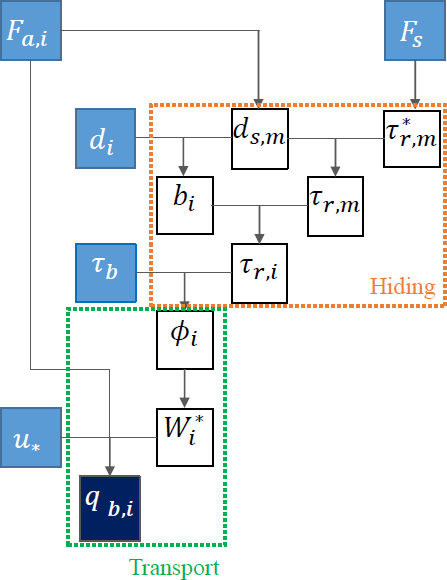
\includegraphics[scale=0.5]{./graphics/Wilcock_application}%
\caption{Scheme of application of the graded sediment transport model of WC-2003. Parameters in blue boxes are input parameters, those in white boxes are intermediary variables computed to estimate the transport rate of size fraction $i$ in the black box.}%
\label{fig:Wilcock_Application}
\end{figure}

Further details on the WC-2003 formula and applications can be found in~\cite{Cordieretal_2019,CORDIER2020103580}.

\noindent

\subsubsection{Engelund-Hansen}
\begin{itemize}
 \item \telkey{BED-LOAD TRANSPORT FORMULA FOR ALL SANDS = 30}
 \item The dimensionless current-induced sediment transport rate is given by:
  \begin{equation*}
  \Phi_b=0.1 \frac{\theta^{\frac{5}{2}}}{c_f}
  \end{equation*}
 with $c_f$ the adimensional friction coefficient and $\theta$ the Shields number without the correction factor for skin friction ($\theta=\frac{\tau_b}{(\rho_s-\rho)gd}$).
 \item Fortran subroutine {\ttfamily bedload\_engel.f}.
\end{itemize}
An exhaustive revision of some common bedload transport formulas and associated information presented in chronological order of development can be found in Table D-2 of~\cite{GarciaBook2006}.
%...............................................................................
\subsection{Modification of the magnitude and direction of bedload}\label{sec:corrections}
%...............................................................................
Three key aspects must be considered for computing the magnitude and direction of the bed load~\cite{Abad08}:
\begin{itemize}
\item[(a)] The effect of the local bed slope
\item[(b)] Secondary flow effects on the direction of the bed shear stress, also refered as to helical flows in the literature
\item[(c)] The bed shear stress partitioning into components affected by skin friction and drag force from bedforms
\end{itemize}
\noindent
\gaia{} includes methods for evaluating these three aspects.

\begin{figure}[H]%
\begin{center}
  \begin{tabular}{ccc}
    \subfloat[]{
      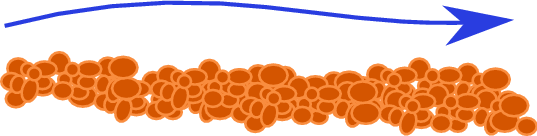
\includegraphics[scale=0.25]{./graphics/transport_1}}&
    \subfloat[]{
      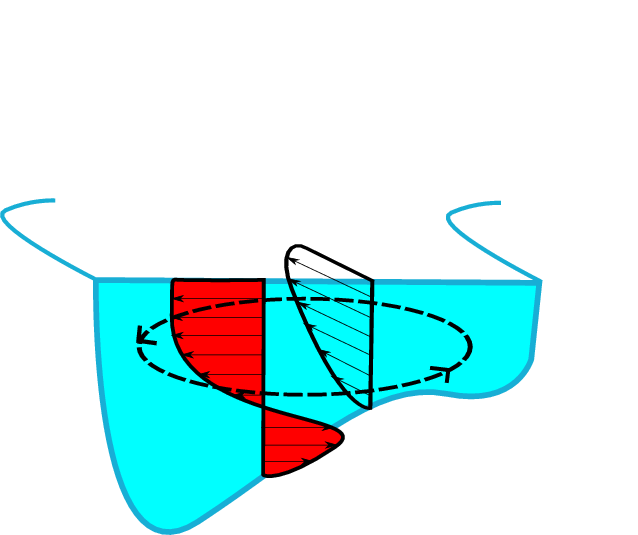
\includegraphics[scale=0.20]{./graphics/curve_4}}&
    \subfloat[]{

\includegraphics[scale=0.75]{./graphics/dunes_drag_grain}}
\end{tabular}
\end{center}
%\caption
%{ADD CAPTION\protect.}
\label{fig:ExampleImage}
\end{figure}

%-------------------------------------------------------------------------------
\subsection{Correction of the direction of the sediment transport}
%-------------------------------------------------------------------------------
The angle $\alpha$ is the angle between the sediment transport direction and the $x-$axis direction will deviate from that of the shear stress by combined action of a transverse slope and secondary currents
In a Cartesian coordinate system, the relation of van Bendegon is:


\begin{minipage}{0.5\textwidth}
\centering
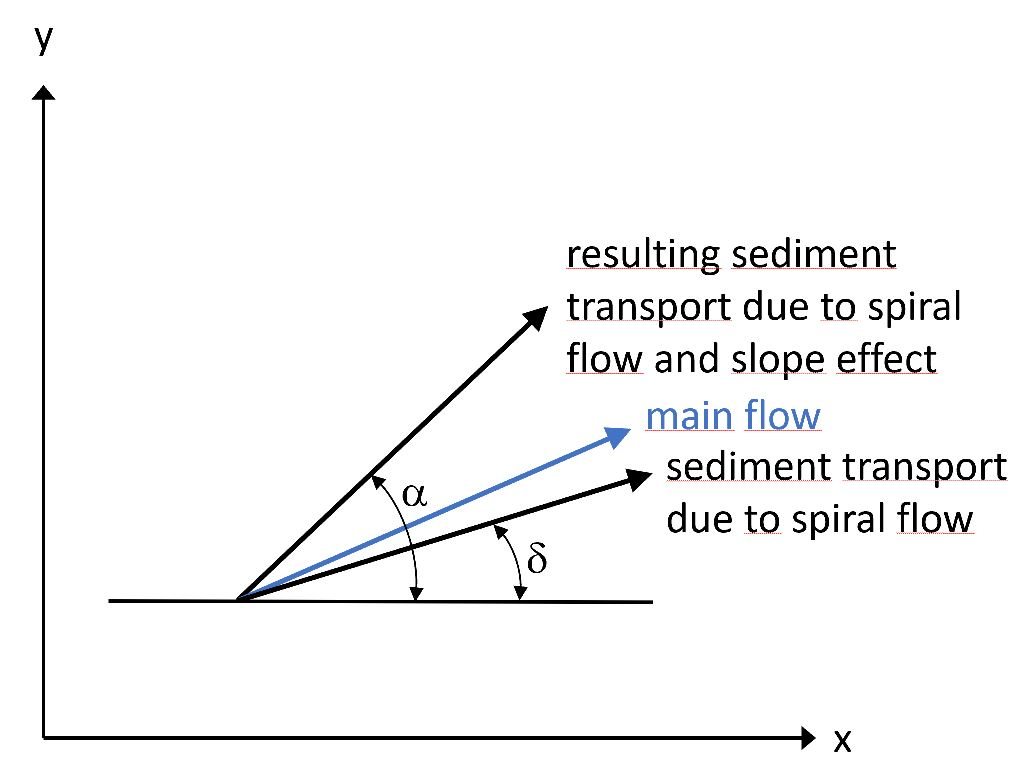
\includegraphics[scale=0.5]{./graphics/sketch_direction_sediment.jpg}%
\end{minipage}
\begin{minipage}{0.5\textwidth}
\begin{equation}
\displaystyle
\tan\alpha = \frac{\sin\delta-\frac{1}{f(\theta)}\frac{\partial z_b}{\partial y}}{\cos\delta-\frac{1}{f(\theta)}\frac{\partial z_b}{\partial x}}.
\end{equation}
\end{minipage}


Above, the terms $\partial z_b/\partial x$ and $\partial z_b/\partial y$ represent respectively the transverse and longitudinal slopes, $z_b$ the bottom position and $\delta$ the angle
between the cartesian coordinate system and the spiral flow. The sediment shape function $f(\theta)$ is a function weighting the influence of the transverse bed slope, expressed as a function of the non-dimensional shear stress or Shields parameter $\theta$. It can be computed according to:

\begin{itemize}
\item Koch and Flokstra~\cite{KochFlokstra80}:
\begin{equation*}
f(\theta) = \frac{3}{2\theta}
\end{equation*}
\item Talmon \textit{et al.}~\cite{Talmon95}:
\begin{equation*}
f(\theta) = \beta_2\sqrt{\theta}
\end{equation*}
where $\beta_2$ is an empirical coefficient. The default value is $\beta_2=0.85$, but an optimal value of $\beta_2=1.6$ was found for the calibration of numerical experiments of dunes and bars in a laboratory channel~\cite{Mendoza15}.
\item Apsley and Stansby~\cite{ApsleyStansby2008}:
\begin{equation*}
f = \frac{\theta_{cr} \cos^2\chi}{\tan\phi}
\end{equation*}
where the slope angle $\cos\chi$ is calculated from the $x$- and $y$-components
of the bed gradient $\cos\chi = 1/\sqrt{1 + (\partial z/\partial x)^2 + (\partial z/\partial y)^2}$ and $\phi$ is the angle of repose.

\end{itemize}

%-------------------------------------------------------------------------------
\subsection{Correction by secondary flow effects on the direction of the bed shear stress}
%-------------------------------------------------------------------------------
In curved channels, the direction of the sediment transport will no longer coincides with the direction of the bed shear stress,
due to the effect of the secondary flows:
\begin{equation}\label{eq:delta}
\delta = \tan^{-1}\left(\frac{v}{u}\right) - \textcolor{red}{\tan^{-1}\left(\frac{A}{r_s}h\right)} = \delta^* - \textcolor{red}{\Delta\delta},
\end{equation}
with $h$ the water depth, $(u,v)$ the components of the depth-averaged velocity field, $r_s$ the local radius of curvature and $A$ the spiral flow coefficient. Above, the term highlighted in red accounts for the effect of the spiral motion on the sediment flux. The angles $\delta^*$ and $\Delta\delta$ indicate respectively the direction of the bed shear stress (which coincides with the direction of the depth-averaged velocity) and the direction due to the effect of secondary currents.

In \gaia{} $A=7^*$ (Engelund's value). Nevertheless, an optimal value of $A=12$ was found for the calibration of numerical experiments of dunes and bars in a laboratory channel~\cite{Mendoza15}.

%-------------------------------------------------------------------------------
\subsection{Correction of the magnitude of the sediment transport}
%-------------------------------------------------------------------------------
The correction of the magnitude of the sediment transport can be computed according to:
\begin{itemize}
\item  Koch and Flokstra~\cite{KochFlokstra80} which is based on the modification of the bed load transport rate by a factor that acts as a diffusion term in the bed evolution equation
\begin{equation}
\begin{array}{ll} \displaystyle
Q_b^* &= Q_{b}\left(1+\beta\frac{\partial z_b}{\partial s}\right) \\
    &= Q_{b}\left[1 + \beta \left(\frac{\partial z_b}{\partial x} \cos\alpha + \frac{\partial z_b}{\partial y} \sin\alpha\right)\right],
\end{array}
\end{equation}
where $s$ is the flow direction and $\beta$ is an empirical factor accounting for the streamwise bed slope effect ($=1.3$ by default).
\medskip

\item Soulsby~\cite{Soulsby97} which s based on the modification of the critical Shields parameter and is therefore only valid for threshold bedload formulas:
\begin{equation*}
\frac{\theta_{\beta cr}}{\theta_{cr}} = \frac{\cos\psi \sin\chi +
\sqrt{\cos^2\chi \tan^2\phi - \sin^2\psi \sin^2\chi}}{\tan
\phi}
\end{equation*}
where $\theta_{\beta cr}$ is the corrected  Shields number for a sloping bed, $\theta_{cr}$ is the critical Shields number for a flat, horizontal bed, $\phi$ is the angle of repose of the sediment, $\chi$ is the bed slope angle with the horizontal, and $\psi$ is the angle between the flow and the bed slope directions.
\medskip

\item  Apsely and Stansby~\cite{ApsleyStansby2008} which is  based on the modification of the critical Shields parameter $\theta_{\beta cr}$ and on the calculation of a effective dimensionless shear stress $\theta_{beta}$.
The modification of the critical shear stress can only be done for threshold bedload formulas. The modification of the Shields parameter $\theta_{\beta}$ could be done for all bedload formulas which are using the shear stress and accordingly the Shields parameter. But it is not recommended.
\begin{equation*}
\frac{\theta_{\beta cr}}{\theta_{cr}} = \cos\chi = 1 / \sqrt{1 + (\partial z /\partial x)^2 + (\partial z/ \partial y)^2 }
\end{equation*}

\begin{equation*}
\theta_{\beta} = \sqrt{\left( \theta \cos\gamma - \frac{\theta_{cr}}{\tan\phi} \frac{\partial z}{\partial x} \cos^2 \chi \right)^2 +
\left(\theta \sin\gamma - \frac{\theta_{cr} }{\tan\phi} \frac{\partial z}{\partial y} \cos^2 \chi \right)^2 }
\end{equation*}
where $\gamma$ is the direction of the bed shear stress.
\end{itemize}



%-------------------------------------------------------------------------------
\subsubsection{Sediment sliding}
%-------------------------------------------------------------------------------
If the bottom slope is higher than a critical slope (typically the angle of repose) sediments can be moved due to geomechanical processes. In \gaia{} two formulas are implemented to calculate sediment displacement in down-slope direction only driven by the bottom slope.
\begin{itemize}

\item The first method is a simple and mass conservative smoothing of the bottom slopes. The changed masses are balanced separately in the mass-balance (MASS EVOLUTION DUE TO SLIDING FORMULA 1).

\item Apsely and Stansby~\cite{ApsleyStansby2008} provide a formulation of avalanching if the bed slope is higher than the angle of repose. In this case the bedload flux  is increased by an additional contribution $q_{aval}$ in the direction of the highest bottom slope. This formula changes the intensity and the direction of the bed load.

\begin{equation*}
q_{aval} = (1-p)\frac{\frac{1}{2} L^2 (\tan\chi - \tan\phi)}{\cos\chi \Delta t}\qquad  \textrm{if} \enspace \tan\chi> \tan\phi
\end{equation*}
\end{itemize}
%-------------------------------------------------------------------------------
\subsection{Keywords for the modification of the intensity and direction of bed load}
%-------------------------------------------------------------------------------
The keyword \telkey{SLOPE EFFECT} (logical type variable, set to {\ttfamily = YES} by default) activates the bed slope effects. If \telkey{SLOPE EFFECT = NO}, the keywords \telkey{FORMULA FOR DEVIATION} and \telkey{FORMULA FOR SLOPE EFFECT} are not taken into account.

%-------------------------------------------------------------------------------
\subsubsection{Correction of the direction of bedload transport}
%-------------------------------------------------------------------------------
The correction of the direction of bedload transport can be done by
\begin{itemize}
\item the Koch and Flokstra formulation \telkey{FORMULA FOR DEVIATION = 1} (integer type variable, set to {\ttfamily = 1} by default),
\item the Talmon et al. formulation \telkey{FORMULA FOR DEVIATION = 2}. This keyword has the associated keyword \telkey{PARAMETER FOR DEVIATION} (real type variable named \telkey{BETA2}, set to {\ttfamily = 0.85} by default).
\item the Apsley and Stansby formulation  \telkey{FORMULA FOR DEVIATION = 3}. This keyword has the associated keyword \telkey{FRICTION ANGLE OF THE SEDIMENT} (real type variable, set to {\ttfamily = 40} by default) and the critical Shields parameter which is calculated by default or can be set with the keyword \telkey{CLASSES SHIELDS PARAMETERS}.
\end{itemize}

%-------------------------------------------------------------------------------
\subsubsection{Correction of the intensity of bedload transport rate}
%-------------------------------------------------------------------------------
The correction of the intensity of bedload transport rate can be done by :
\begin{itemize}
\item the Koch and Flokstra formulation \telkey{FORMULA FOR SLOPE EFFECT} (integer type variable, set to {\ttfamily = 1} by default). This keyword has the associated keyword \telkey{BETA} (real type variable, set to {\ttfamily = 1.30} by default)
\item the Soulsby formulation \telkey{FORMULA FOR SLOPE EFFECT = 2}. This keyword has the associated keyword \telkey{FRICTION ANGLE OF THE SEDIMENT} (real type variable, set to {\ttfamily = 40.} by default) and the critical Shields parameter which is calculated by default or can be set with the keyword \telkey{CLASSES SHIELDS PARAMETERS}.
\item the Apsley and Stansby formulation \telkey{FORMULA FOR SLOPE EFFECT = 3}. This keyword has the associated keyword \telkey{FRICTION ANGLE OF THE SEDIMENT} (real type variable, set to {\ttfamily = 40} by default) and the critical Shields parameter which is calculated by default or can be set with the keyword \telkey{CLASSES SHIELDS PARAMETERS}.
\end{itemize}

%-------------------------------------------------------------------------------
\subsubsection{Correction due to secondary currents}
%-------------------------------------------------------------------------------
The keyword \telkey{SECONDARY CURRENTS} (logical type variable, set to {\ttfamily = NO} by default) accounts for the secondary flow correction. This keyword has the associated keyword \telkey{ SECONDARY CURRENTS ALPHA COEFFICIENT} (real type variable, set to {\ttfamily = 1.} by default) that allows the modification of the coefficient $A$ in Equation~\ref{eq:delta}. This value can be chosen as: $\rightarrow 0.75~~\text{(rough bottom)} \leq \alpha_{SC} \leq 1.0~~\text{(smooth bottom)}$. For example, if $\alpha_{SC} = 1$ then $A = 7$.

%-------------------------------------------------------------------------------
\subsubsection{Correction due to sediment sliding}
%-------------------------------------------------------------------------------
Sediment sliding will be taken into account if the keyword \telkey{SEDIMENT SLIDE}
(integer type variable, set to {\ttfamily = 0} by default) is higher zero:
\begin{itemize}
\item  \telkey{SEDIMENT SLIDE = 1} smoothes the bottom slopes up to the angle of repose.
\item  \telkey{SEDIMENT SLIDE = 2} calculates the sediment sliding with the avalanching formula from Apsley and Stansby.
\end{itemize}
This keyword has the associated keyword \telkey{FRICTION ANGLE OF THE SEDIMENT} (real type variable, set to {\ttfamily = 40} by default)

%-------------------------------------------------------------------------------
\subsection{Influence of the roughness on sediment transport processes}\label{sec:roug}
%-------------------------------------------------------------------------------
%-------------------------------------------------------------------------------
\subsubsection{Skin friction correction}\label{sec:skin}
%-------------------------------------------------------------------------------
The total bed shear stress is due to skin friction and bed form drag but \textbf{only the component due to skin friction acts on bedload}. The shear stress due to skin friction is expressed as:
\begin{equation}\label{eq:taup}
\tau'=\mu\tau_b,
\end{equation}
where $\tau_b = 0.5 \rho C_f (U^2 + V^2)$ is the total bed shear stress and $\mu$ is the friction factor:
\begin{equation}\label{eq:mu}
\mu=\frac{C_f'}{C_f}
\end{equation}
where $C_f$ is the friction coefficient due to form drag plus skin friction (specified in the hydrodynamics module), and $C_f'$ is the friction coefficient due only to skin friction, which is computed as:
\begin{equation}\label{eq:cfp}
C_f'=2\left(\frac{\kappa}{\log(12h/k_s')}\right)^2,
\end{equation}
where $\kappa$ is the von K\'arm\'an coefficient ($=0.40$), the roughness height $k_s'=\alpha_{k_s}d_{50}$, the coefficient $\alpha_{k_s}$ is a calibration parameter.

%-------------------------------------------------------------------------------
\subsubsection{Keywords for skin friction correction}
%-------------------------------------------------------------------------------
The keyword \telkey{SKIN FRICTION CORRECTION} (integer type variable, {\ttfamily = 1} by default) activates the correction of the bed shear stress due to skin friction:
\begin{itemize}
\item If \telkey{SKIN FRICTION CORRECTION = 0}, then $\mu=1$ and the total bed shear stress issued from the hydrodynamics computation is used
\item If \telkey{SKIN FRICTION CORRECTION = 1}, $\mu$ is computed according to Equation~\ref{eq:mu}. In this case, the friction coefficient $C_f$ is provided by the hydrodynamics steering file and $C_f'$ is computed by Equation~\ref{eq:cfp}. To compute $k_s'=\alpha_{k_s} d_{50}$, the coefficient $\alpha_{k_s}$ can be modified with the keyword \telkey{RATIO BETWEEN SKIN FRICTION AND MEAN DIAMETER} (real type variable, {\ttfamily = 3.} by default). In the numerical experiments of Mendoza \textit{et al.}~\cite{Mendoza15}, $\alpha_{k_s}=37$ for dunes and $\alpha_{k_s}=3.6$ for bars.

 \begin{WarningBlock}{Note:}
  By default, the keyword \telkey{SKIN FRICTION CORRECTION = 1}. In the presence of very shallow waters, this correction can present stability issues. For this case, we suggest the user to set the keyword \telkey{SKIN FRICTION CORRECTION = 0}.
  \end{WarningBlock}

\item If \telkey{SKIN FRICTION CORRECTION = 2}, the presence of ripples is taken into account to compute $\mu$ (see subroutine \texttt{tob\_gaia.f}). For this option, a bedform predictor is used to calculate the bedform roughness $k_r$ in order to account for the effect of ripples. Both $k_r$
and $k_s'$ should influence the transport rates. It is assumed that:
\begin{equation}\label{eq:mu2}
\mu =\frac{C_f'^{0.75} C_r^{0.25}}{C_f},
\end{equation}
where the quadratic friction $C_r$ due to bedforms is calculated as a
function of $k_r$ (see \S~\ref{sec:bedroughpredictor}).
\end{itemize}

%-------------------------------------------------------------------------------
\subsection{Bed roughness predictor}\label{sec:bedroughpredictor}
%-------------------------------------------------------------------------------
A natural sediment bed is generally covered with bedforms, with length $\lambda_d$ (m)
and height $\eta_d$ (m). The presence of bed forms greatly modifies the boundary
layer flow structure, with the formation of recirculation cells and
depressions in the lee of bedforms.\\

Depending on the flow and sediment transport rates, the size of bed
forms ranges from a few centimeters for ripples to a few tens of meter for
mega-ripples. The dimension of dunes scales with the water depth $h$, such that $\eta_d
\approx 0.4 h$ and  $\lambda_d\approx [6-10] h$.\\

In most cases, large scale models do not resolve the small to medium
scale bedforms (such as ripples or mega-ripples) which need therefore to be parameterized by increasing the friction coefficient. To determine bed roughness, there are two options available in \gaia{}:
\begin{itemize}
\item By imposing the friction coefficient based on friction laws: in this case the values of the friction coefficients are provided by \telemac{2D} or \telemac{3D}.
\item By predicting the value of the bed roughness as a function of flow and sediment parameters using a bed roughness predictor. This option is discussed below.
\end{itemize}
Different options are programmed in \gaia to predict the total bed
roughness through the associated keywords \telkey{COMPUTE BED ROUGHNESS AT SEDIMENT SCALE} (logical type variable, set to {\ttfamily = NO} by default) and \telkey{BED ROUGHNESS PREDICTOR OPTION}. The calculated Nikuradse value for the total bed roughness is given to the hydrodynamics. Therefore, the Nikuradse friction law must be selected in the hydrodynamics. The roughness coefficient of the hydrodynamic is only changed for nodes with movable bed.
% no stand alone option for GAIA anymore!
%It is recalled that the bed friction option of \gaia is not
%used in the case of internal coupling with \telemac{2D} or \telemac{3D}.
\begin{itemize}
\item For {\ttfamily BED ROUGHNESS PREDICTOR OPTION = 1}: the bed is assumed to be flat $k_s = k_s'= \alpha_{k_s} d_{50}$, with $\alpha_{k_s}$ a constant (assumed to be equal to $3.$), modified by the keyword \telkey{RATIO BETWEEN SKIN FRICTION AND MEAN DIAMETER}.
\item {\ttfamily BED ROUGHNESS PREDICTOR OPTION = 2}: the bed is assumed to be covered by ripples.
  \begin{itemize}
    \item For currents only, the ripple bed roughness is function of the mobility number, see~\cite{vanRijn07}:
\begin{equation*}
k_r =\left\{\begin{array}{ll}
d_{50}(85-65\tanh(0.015(\Psi-150))) & \text{for\,} \Psi<250\\
20 d_{50} & \text{otherwise}
\end{array}
\right.
\end{equation*}
with $\Psi =U^2/(s-1)gd_{50}$.

    \item For waves and combined waves and currents, bedform dimensions are calculated
as a function of wave parameters following the method of Wiberg and Harris~\cite{WibergHarris}.
The wave-induced bedform bed roughness $k_r$ is calculated as a function of the wave-induced bedform
height $\eta_r$:
\begin{equation}
k_r = \max(k_s', \eta_r).
\end{equation}
Then $k_s=k_s'+k_r$.
  \end{itemize}

\item {\ttfamily BED ROUGHNESS PREDICTOR OPTION = 3}: for currents only, the van Rijn's total bed roughness predictor~\cite{vanRijn07, Huybrechts} has been implemented.
The total bed roughness can be decomposed into a grain
roughness $k_s'$, a small-scale ripple roughness $k_r$, a mega-ripple
component $k_{mr}$, and a dune roughness $k_d$:
\begin{equation}\label{eq:totalbedroughness}
k_s = k_s' + \sqrt{k_r^2 + k_{mr}^2 + k_d^2}.
\end{equation}
Both small scale ripples and grain roughness have an influence on the
sediment transport laws, while the mega-ripples and dune roughness only
contribute to the hydrodynamic model (total friction). In Equation~\ref{eq:totalbedroughness}, the general expression for megaripples roughness $k_{mr}$ is given by:
\begin{equation}
k_{mr} = 0.00002\,f_{ts}\,h\,(1-\exp^{-0.05\Psi})\,(550-\Psi),
\end{equation}
with
\begin{equation*}
f_{ts} =\left\{\begin{array}{ll}
d_{50}/(1.5d_{sand}) & \text{for\,} d_{50}\leq 1.5d_{sand}\\
1.0 & \text{otherwise}
\end{array}
\right.
\end{equation*}
and the general expression for dune roughness $k_d=0.00008\,f_{ts}\,h\,(1-\exp^{-0.02\Psi})\,(600-\Psi)$.

\end{itemize}

%-------------------------------------------------------------------------------
\subsection{Boundary conditions for bedload}
%-------------------------------------------------------------------------------
The specification of boundary conditions is done in a boundary condition file, usually named with extension \texttt{*.cli}. The reader is referred to \S\ref{sec:flags} for the definition of the different flags used in the boundary condition file.

\subsubsection{Wall boundary conditions}
At banks and islands, the bedload transport rate is set to zero. For this case, the flag \texttt{LIEBOR} is set \texttt{= 2} as shown in the example below:

\begin{lstlisting}[frame=trBL]
2 2 2 0.0 0.0 0.0 0.0 (*@\color{PantoneRed}2@*) 0.0 0.0 0.0 565 1
\end{lstlisting}

\subsection{Inflow boundary conditions}
In a depth-averaged 2D sediment transport model, the sediment discharge must be given at each point of the inflow boundary. The different cases can be present:
\subsubsection{Equilibrium sediment discharge}
For this case, the flag \texttt{LIEBOR} is set \texttt{= 5} and the flag \texttt{EBOR} is set \texttt{= 0.0} (no bottom change at the inflow boundary) as shown in the example below:

\begin{lstlisting}[frame=trBL]
4 5 5 0.0 0.0 0.0 0.0 (*@\color{PantoneRed}5@*) (*@\color{PantoneRed}0.0@*) 0.0 0.0 565 1
\end{lstlisting}

\subsubsection{Constant sediment discharge in time}
For this case, boundary condition files are needed for both \telemac{2D} and \gaia{}. In the \gaia{}'s boundary condition file, the flag \texttt{LIQBOR = 5} and \texttt{LIEBOR = 4}. The imposed solid discharge can be specified as follows:
\begin{itemize}
\item A value of the unit solid discharge [kg/(m~s)] in the column \texttt{Q2BOR} of the \gaia{}'s boundary condition file, as shown in the example below for an imposed unit discharge \texttt{Q2BOR=}$1.0$~kg/(m~s):
\begin{lstlisting}[frame=trBL]
4 (*@\color{PantoneRed}5@*) 5 (*@\color{PantoneRed}1.0@*) 0.0 0.0 0.0 (*@\color{PantoneRed}4@*) 0.0 0.0 0.0 565 1
\end{lstlisting}

Particular cases of \texttt{Q2BOR} can be programmed in the subroutine \texttt{conlit.f}.

\item A value of the total solid discharge (without pores) [kg/s] given through the keyword \telkey{PRESCRIBED SOLID DISCHARGES} (sequence of real values separated by semi-colons, one value per liquid boundary, no default value) in the steering file, as shown in the example below for an imposed total discharge equal to $10.0$~kg/s:
\begin{lstlisting}[frame=trBL]
4 (*@\color{PantoneRed}5@*) 5 1.0 0.0 0.0 0.0 (*@\color{PantoneRed}4@*) 0.0 0.0 0.0 565 1
\end{lstlisting}
\begin{lstlisting}[frame=trBL]
PRESCRIBED SOLID DISCHARGES : 10.0
\end{lstlisting}
When a value of solid discharge is given in the parameter file, \texttt{Q2BOR} is considered as only a profile (so it must be greater than 0.). For a constat profile, values equal to 1.0 (as here above) must be filled in.

\end{itemize}

\subsubsection{Time-series of sediment discharge}
Time-series values of sediment discharge are specified in a file through the keyword \telkey{LIQUID BOUNDARIES FILE} (character type), declared in the hydrodynamic steering file. The \gaia{}'s boundary condition file must contain the flags as shown below:
\begin{lstlisting}[frame=trBL]
4 (*@\color{PantoneRed}5@*) 5 1.0 0.0 0.0 0.0 (*@\color{PantoneRed}4@*) 0.0 0.0 0.0 565 1
\end{lstlisting}

The keyword \telkey{PRESCRIBED SOLID DISCHARGES} must be also included in the steering file, with an arbitrary value.

\subsubsection{Repartition of imposed sediment discharge in case of graded
distributions}
In case of several classes of non-cohesive sediments, the sediment discharge can
 be subdivided to the various classes through the keyword
\telkey{CLASSES IMPOSED SOLID DISCHARGES DISTRIBUTION} (sequence of real values
separated by
semi-colons, one value per class whose sum is equal to 1.).

In cases where this keyword is not used, the sediment discharge will be
subdiveded among the various classes according to the sand ratio computed
by \gaia.

\subsection{Outflow boundary conditions}
At the outflow boundary, bedload does not require any particular boundary condition.
For this case, the flag \texttt{LIEBOR} is set \texttt{= 4} as shown in the example below:

\begin{lstlisting}[frame=trBL]
5 4 4 0.0 0.0 0.0 0.0 (*@\color{PantoneRed}4@*) 0.0 0.0 0.0 565 1
\end{lstlisting}

%-------------------------------------------------------------------------------
\subsection{Useful graphical printouts for bedload}
%-------------------------------------------------------------------------------
Through the keyword \telkey{ VARIABLES FOR GRAPHIC PRINTOUTS}, some useful printouts for bedload sediment transport are listed below:
\begin{lstlisting}[frame=trBL]
TOB="Bed shear stress(N/m2)";
MU ="Skin friction coefficient";
M="bed-load discharge (kg/(m*s)";
N="bed-load discharge along x axis (kg/(m*s))";
P="bed-load discharge along y axis (kg/(m*s))";
E="bottom evolution (m)";
QSBL="bed load transport rate (kg/(m*s))";
\end{lstlisting}

\begin{WarningBlock}{Note:}
The sediment discharge is the mass of sedimentary material, both particulate and dissolved, that passes across a given flow-transverse cross section of a given flow in unit time. The flag {\ttfamily M} accounts for the total solid discharge (bedload plus suspended load), while {\ttfamily QSBL} accounts for the bed load solid discharge. If suspended load is not taken into account in the simulation, the output values of {\ttfamily M} and {\ttfamily QSBL} are equivalent.
\end{WarningBlock}
%-------------------------------------------------------------------------------
\subsection{Useful graphical printouts for continuing a computation}
%-------------------------------------------------------------------------------
As for the module \telemac{2D}, in \gaia{} it is possible to continue a computation, taking a time step of a previous computation, on the same mesh as initial state.
As well as for the hydrodynamic part, it is necessary to declare two keywords in the steering file:
\begin{enumerate}
\item \telkey{COMPUTATION CONTINUED}, which must be set equal to YES
\item \telkey{PREVIOUS SEDIMENTOLOGICAL COMPUTATION FILE}, to give the name of the file that will supply the initial state.
\end{enumerate}
When continuing a computation it is important that the previous sedimentological computation file contains the appropriate variables in order to properly continue the computation. Below some advices are introduced:

\begin{WarningBlock}{Note:}
\begin{itemize}
\item the bottom (B) and the layer thickness (*ES) are mandatory
\item the non erodable bottom (R) is optional since when missing, it is computed using the layer thickness
\item the masses are mandatory to continue the computation, so:
\begin{itemize}
 \item if the variables *S* (or *M*) are saved in the previous file, they will be directly taken for continuing computation
 \item if the previous file does not contain masses, they will be reconstructed using the ratios (*A*,*R*) and the porosity, as well as the thickness.
\end{itemize}
\end{itemize}
\end{WarningBlock}

These suggestions are necessary only when the
\telkey{PREVIOUS SEDIMENTOLOGICAL COMPUTATION FILE} is manually generated by
users (as result file of a previous computation).
Indeed, since release v8.5, the new feature \telkey{RESTART MODE} for \gaia{}
has been introduced and described in \ref{sec-restart} to facilitate computation
continuing when using \gaia{}.

%
%the following is to do
%-------------------------------------------------------------------------------
%\subsection{Non-uniform sediment distribution}
%-------------------------------------------------------------------------------
